%(BEGIN_QUESTION)
% Copyright 2006, Tony R. Kuphaldt, released under the Creative Commons Attribution License (v 1.0)
% This means you may do almost anything with this work of mine, so long as you give me proper credit

Bestem temperaturen i måleskjøten i denne termoelementkretsen (type K), gitt referanseskjøttemperatur og voltmeterutslag. Avrund svaret til nærmeste hele grad Fahrenheit:

$$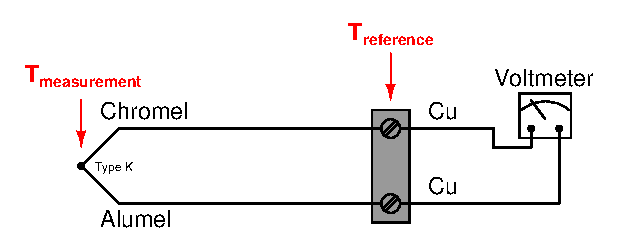
\includegraphics[width=15.5cm]{i00382x01.eps}$$

\begin{itemize}
\item{} $T_{reference}$ = 70$^{o}$ F ; voltmeterspenning = 20.018 mV ; $T_{measurement}$ = ???
\item{} $T_{reference}$ = 65$^{o}$ F ; voltmeterspenning = 5.833 mV ; $T_{measurement}$ = ???
\item{} $T_{reference}$ = 52$^{o}$ F ; voltmeterspenning = 31.420 mV ; $T_{measurement}$ = ???
\item{} $T_{reference}$ = 73$^{o}$ F ; voltmeterspenning = $-$2.027 mV; $T_{measurement}$ = ???
\end{itemize}

\vskip 20pt \vbox{\hrule \hbox{\strut \vrule{} {\bf Forslag til sokratisk diskusjon} \vrule} \hrule}

\begin{itemize}
\item{} For RTD-er kan man bruke formel for sammenheng mellom motstand og temperatur i stedet for tabell. Tror du det også er mulig for termoelementer? Hvis ja, hvordan kan en spenning/temperatur-formel se ut?
\end{itemize}

\underbar{file i00382}
%(END_QUESTION)





%(BEGIN_ANSWER)

\noindent
{\bf Delvis svar:}

\begin{itemize}
\item{} $T_{reference}$ = 70$^{o}$ F ; voltmeterspenning = 20.018 mV ; $T_{measurement}$ = 941 $^{o}$F
\item{} $T_{reference}$ = 73$^{o}$ F ; voltmeterspenning = $-$2.027 mV; $T_{measurement}$ = $-$20 $^{o}$F
\end{itemize}

%(END_ANSWER)





%(BEGIN_NOTES)

(Fra ITS-90 termoelementtabell:)

\begin{itemize}
\item{} $T_{ref}$ = 70$^{o}$ F ($V_{ref}$ = 0.843 mV); $V_{meter}$ = 20.018 mV ; {\bf $T_{meas}$ = 941$^{o}$ F ($V_{meas}$ = 20.861 mV)}
\item{} $T_{ref}$ = 65$^{o}$ F ($V_{ref}$ = 0.731 mV) ; $V_{meter}$ = 5.833 mV ; {\bf $T_{meas}$ = 321$^{o}$ F ($V_{meas}$ = 6.564 mV)}
\item{} $T_{ref}$ = 52$^{o}$ F ($V_{ref}$ = 0.441 mV); $V_{meter}$ = 31.420 mV ; {\bf $T_{meas}$ = 1410$^{o}$ F ($V_{meas}$ = 31.861 mV)}
\item{} $T_{ref}$ = 73$^{o}$ F ($V_{ref}$ = 0.910 mV) ; $V_{meter}$ = $-$2.027 mV; {\bf $T_{meas}$ = $-$20$^{o}$ F ($V_{meas}$ = $-$1.117 mV)}
\end{itemize}




\vfil \eject

\noindent
{\bf Oppsummeringsquiz:}

Bruk termoelementtabell (ITS-90), og bestem temperaturen for et type J-termoelement (måleskjøt) når voltmeteret viser 14.843 mV og omgivelsestemperaturen ved voltmeterledningenes tilkobling er 64 $^{o}$F:

\begin{itemize}
\item{} 524 $^{o}$F
\vskip 5pt
\item{} 493 $^{o}$F
\vskip 5pt
\item{} 553 $^{o}$F
\vskip 5pt
\item{} 479 $^{o}$F
\vskip 5pt
\item{} 494 $^{o}$F
\vskip 5pt
\item{} 555 $^{o}$F
\end{itemize}


%INDEX% Measurement, temperature: thermocouple

%(END_NOTES)
